% THIS IS AN EXAMPLE DOCUMENT FOR VLDB 2010
% based on ACM SIGPROC-SP.TEX VERSION 2.7
% Modified by  Gerald Weber <gerald@cs.auckland.ac.nz>


% This example *does* use the .bib file (from which the .bbl file
% is produced). REMEMBER HOWEVER: After having produced the .bbl file,
% and prior to final submission, you need to 'insert'  your .bbl file into
% your source .tex file so as to provide ONE 'self-contained' source file.


\documentclass[a4paper,12pt]{report}
\renewcommand{\baselinestretch}{1.5}
%\usepackage[linesnumbered,boxed]{algorithm2e}
\usepackage{amsmath}
\usepackage{amsthm}
\usepackage{algorithm}
\usepackage{algorithmic}
%\usepackage{algpseudocode}
\usepackage{graphicx}
\usepackage{verbatim}
\usepackage{latexsym}
\usepackage{subfigure}
\usepackage{subfig}
\usepackage{color}

\usepackage{float}
\usepackage{indentfirst}
\usepackage{wallpaper}
\usepackage{pdfpages}
\usepackage{multirow}
\newtheorem{theorem}{Theorem}
%\usepackage{pdfpages}
%\usepackage{hyperref}
\usepackage{CJK}

\CenterWallPaper{.30}{figure/nthu-logo.pdf}

%set paper size
\special{papersize=8.5in,11in}
\topmargin=14.7mm    %bottom margin 14.7mm
\oddsidemargin=30mm   %left & right margin 17.45mm

%text sizes (Keep these values unchanged!)
\textwidth=150mm \textheight=250mm
\columnsep=5.0mm
\parindent=3.5mm

%misc parameters
\headsep=0mm  \headheight=0mm \footskip=18mm

%conversion to values for LaTeX
\advance\topmargin-1in\advance\oddsidemargin-1in
\evensidemargin\oddsidemargin


\begin{document}

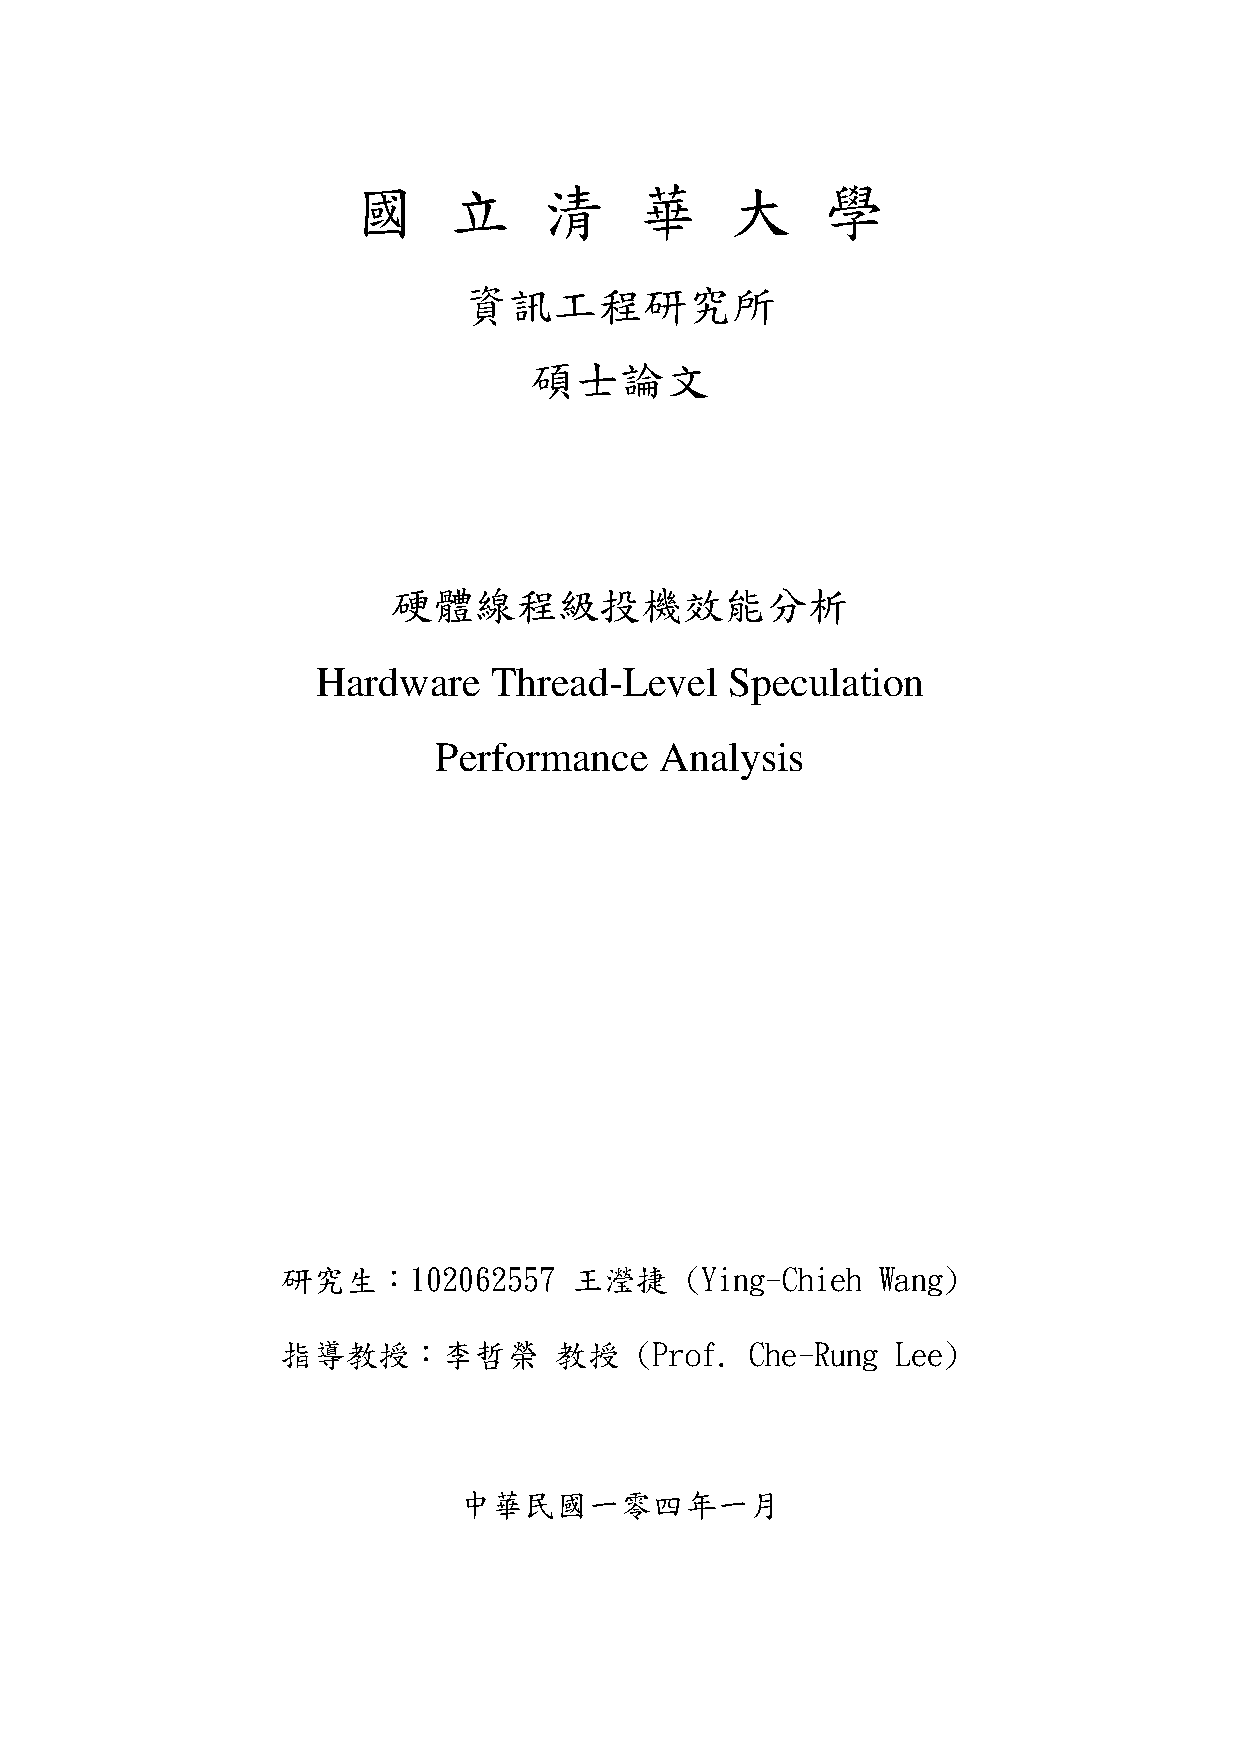
\includepdf[pages={1}]{cover.pdf}
%\includepdf[pages={1}]{cover_ch.pdf}

\title{\bf \huge Hardware Thread-Level Speculation Performance Analysis}
\date{}
\author{
\begin{tabular}{c}
\\
\\
{\LARGE \bf Student: Ying-Chieh Wang}\\
{\LARGE \bf Advisor: Prof. Che-Rung Lee}\\
\\
\\
\\
\\
{\LARGE \bf Department of Computer Science}\\
{\LARGE \bf National Tsing Hua University}\\
{\LARGE \bf Hsinchu, Taiwan, 30013, R.O.C.}\\
\\
{\large January 2015}
\end{tabular}
}

\maketitle
\includepdfset{pagecommand={\thispagestyle{plain}}}

\pagenumbering{roman}
%\addcontentsline{toc}{chapter}{\ctxfr 中文摘要}
\addcontentsline{toc}{chapter}{Chinese Abstract}

\includepdf[pages={1}]{abstract_ch.pdf}

\addcontentsline{toc}{chapter}{Abstract}
\begin{abstract}
\thispagestyle{plain} 
\setcounter{page}{2}
Thread-Level Speculation (TLS) is one of the parallel frameworks. TLS can avoid the analysis problem of compiler-directed code parallelization and this is helpful for programmers to generate parallel programs. However, the performance is the most important issue for parallel programs. Therefore, we analyse the performance of hardware Thread-Level Speculation (TLS) in the IBM Blue Gene/Q computer.

This paper presents a performance model for hardware Thread-Level Speculation (TLS) in the IBM Blue Gene/Q computer. The model shows good performance prediction, as verified by the experiments. The model helps to understand potential gains from using special purpose TLS hardware to accelerate the performance of codes that, in a strict sense, require serial processing to avoid memory conflicts. Based on analysis and measurements of the TLS behavior and its overhead, a strategy is proposed to help utilize this hardware feature. Furthermore, we compare the performance of hardware Thread-Level Speculation and OpenMP. Based on the performance analysis, we give a direction for deciding between this two parallel frameworks. And the results can not only help users to utilize the TLS but also suggest potential improvement for the future TLS architectural designs.
\end{abstract}

% IEEEtran.cls defaults to using nonbold math in the Abstract.
% This preserves the distinction between vectors and scalars. However,
% if the conference you are submitting to favors bold math in the abstract,
% then you can use LaTeX's standard command \boldmath at the very start
% of the abstract to achieve this. Many IEEE journals/conferences frown on
% math in the abstract anyway.

% no keywords



\addcontentsline{toc}{chapter}{Acknowledgements}
\renewcommand{\abstractname}{Acknowledgements}
\begin{abstract}
\thispagestyle{plain}
\setcounter{page}{3}
There are many people giving assistance on my thesis work. I am very grateful to each of them.
Most of all, I would like to show my deepest gratitude to my advisor, Prof. Che-Rung Lee.
Prof. Lee teaches me how to define problems, map out schedule of validation, analyse the result of experiments and do great presentation.
While discussing problems with Prof. Lee, I learned to use mathematical method to solve problems and proofed the results. In addition, Prof. Lee always helps me find the right direction to overcome difficulties. Therefore, I got more progress in study and also be more delighted on doing research.
Except researching, Prof. Lee provided me the chance to train the junior students to attend Student Cluster Competition. I learned a lot and been inspired while I was teaching and discussing with them.

I would like to express thanks to Dr. I-Hsin Chung, a cooperative partner in IBM, he gave me advises on project and help me learn professional knowledge about my research. Except working, Dr. Chung also teached me the importance of relationship and provided me a chance to get a job in IBM.
And My lab mates also support me on my way of research during the two years. They gave me favors anytime I needed helps. I really appreciate scope lab.

My family always encourage me to achieve my best. I am very grateful to my parents and my brother.
Thanks to all the people around me.

\end{abstract} 

\setcounter{page}{4}
\addcontentsline{toc}{chapter}{Contents}
\tableofcontents
\clearpage
\addcontentsline{toc}{chapter}{List of Figures}
\listoffigures
\clearpage
\addcontentsline{toc}{chapter}{List of Tables}
\listoftables
\clearpage
\addcontentsline{toc}{chapter}{List of Algorithms}
\listofalgorithms
\clearpage


\pagenumbering{arabic}
\setcounter{page}{1}
\chapter{Introduction}
\label{chap:intro}
 


\chapter{Background}
\label{chap:background}

As mentioned in previous section, Storm \cite{Aniello:2013:AOS:2488222.2488267} is a real-time, 

\chapter{Conclusion}
\label{chap:conclusion}
This is conclusion.


\bibliographystyle{plain}
\bibliography{note}

% The following two commands are all you need in the
% initial runs of your .tex file to
% produce the bibliography for the citations in your paper.
%{%\scriptsize
%\bibliographystyle{abbrv}
%\bibliography{HPCoC_cite}
%}
% You must have a proper ".bib" file
%  and remember to run:
% latex bibtex latex latex
% to resolve all references

\end{document}
